\section{Introduction}
\label{sec:introduction}

Linear probes are the standard tool for testing what a vision-language model (VLM) represents. They read out a concept by fitting a classifier to activations at a chosen layer \citep{alain2017understanding,belinkov2022probing}. In medical imaging, probes often succeed at linearly decoding clinical findings such as pleural effusion or cardiomegaly from the visual representation of general-purpose and medical VLMs \citep{zhu2026lost,pedersen2026probes}. Activation steering promises the converse: writing the probe direction back into the representation to change the model's behaviour \citep{turner2023steering,panickssery2024caa}. Together, these methods cast the probe direction as a handle on the concept: read it to detect, write it to control. We ask whether that handle exists.

A steering write that changes the answer does not settle the question. In Qwen2.5-VL-7B on NIH ChestX-ray14, a probe reads effusion from the visual tokens the language model consumes, and writing its direction back raises the model's probability of answering yes to the Effusion question by $\cfSeedWEff$, more than the 95th percentile of 119 random directions and a coordinate-permutation sham written at the same dose. By the usual steering criteria, the write works. Writing the Nodule direction into the same patients at the same dose raises the Effusion answer further, by $\cfSeedWNodule$ (Figure~\ref{fig:framework}b, right), although Nodule is the competing direction least similar to Effusion (Appendix~\ref{app:cf-robustness}). Random and sham directions carry no label, so they cannot expose a direction whose effect is shared with other findings \citep{pahde2025navigating}. Exposing it requires writing every competing clinical direction at the same locus and dose in the same patients and asking whether the concept's own direction moves the concept's own answer more than any other. We call the outcome \emph{ownership}. When a concept is readable but not owned, its probe direction reads the concept without writing it: reading is not writing.

We turn this comparison into an evaluation (Section~\ref{sec:framework}, Figure~\ref{fig:framework}). At the \emph{consumed block}, the final visual block whose output the language model reads, each concept receives three grades. It is \emph{readable} if its probe beats random-label probes of equal capacity, \emph{answerable} if the model's yes/no answer without any write beats chance, and \emph{owned} if a fixed-dose write along its direction clears the random and sham references and moves its own answer more than every competing clinical direction does. We apply the evaluation to \cfCheckpoints{} checkpoints from \cfFamiliesWord{} families (3B--72B; general-purpose and medical) on two chest-radiograph datasets with report-derived labels, NIH ChestX-ray14 and CheXpert Plus, and on COCO objects as a natural-image control (Section~\ref{sec:setup}).

On chest radiographs most readable and answerable concepts are not owned, while most COCO objects are, and the gap persists among concepts the model answers well (Section~\ref{sec:results}). We call this gap the \emph{attribution deficit}. Since the same write succeeds on natural images, the remaining results locate the deficit. Checkpoints that share a vision tower write identical vectors into identical representations yet own different concepts, so the model that reads the representation decides ownership. Non-clinical attributes of the same radiographs (projection, sex, and age) are owned no more often than findings, so the deficit does not depend on the concept being clinical. The reader responds to a different direction: a direction fitted to the model's own answers is owned in \cfAnsChestOwnedA{} of \cfAnsChestN{} chest checkpoint--concept cells where the label direction is owned in \cfAnsChestOwnedLabel{}, and on chest radiographs it is nearly orthogonal to the probe direction.

\begin{figure}[t]
    \centering
    \resizebox{\textwidth}{!}{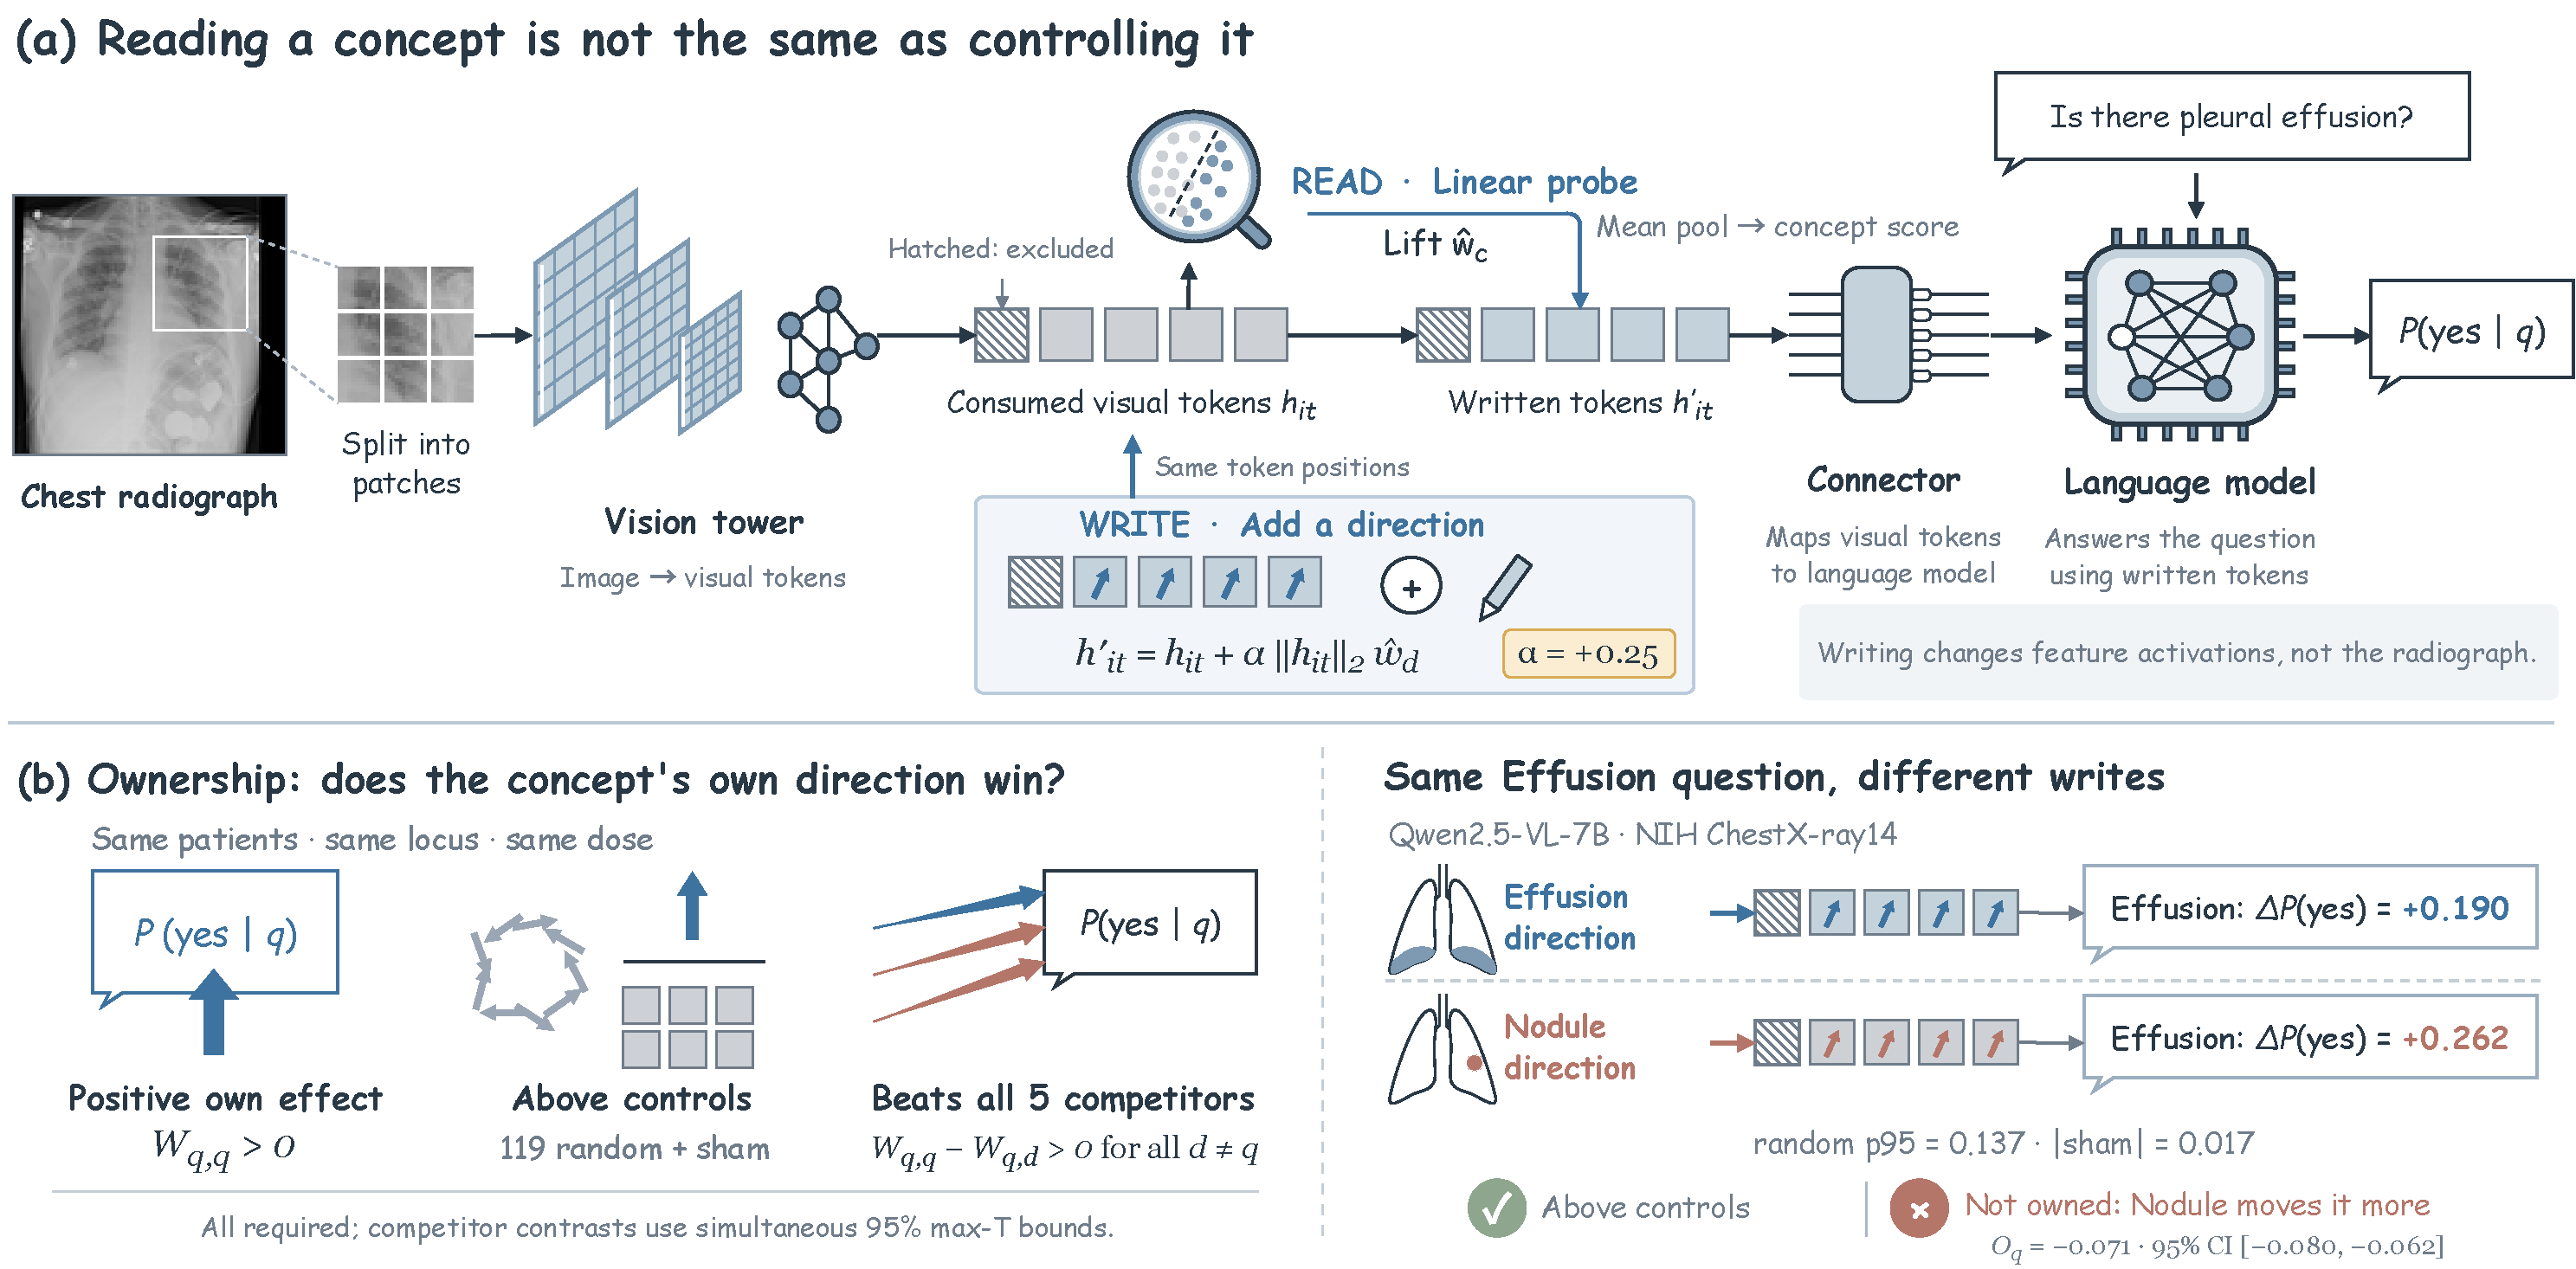
\includegraphics{figures/fig1_framework.pdf}}
    \caption{\textbf{Reading and writing a concept at the consumed block.} (a) The probe reads the concept from the consumed visual tokens, and its lifted normal is written back to them at dose $\alpha=+0.25$, a quarter of each token's norm. (b) Left: the three comparisons that decide ownership, on the write matrix $W_{q,d}$, the mean change in $P(\mathrm{yes})$ of question $q$ under a write along direction $d$. Right: the Effusion case (Qwen2.5-VL-7B, NIH ChestX-ray14): a stronger competitor.}
    \label{fig:framework}
\end{figure}

\paragraph{Contributions.} (i) We introduce ownership, which separates reading a concept from writing it: a probe direction is scored against directions fitted the same way for the competing concepts, written at the same locus and dose in the same patients (Section~\ref{sec:framework}). (ii) We identify the attribution deficit: across \cfCells{} checkpoint--concept cells, clinical concepts on chest radiographs are read and answered far more often than they are owned, and the gap to natural-image objects persists at matched answer ability (Sections~\ref{sec:headline}--\ref{sec:coco}). (iii) We trace the deficit to how the model reads the chest-radiograph representation rather than to the concept's clinical status, and show that a direction fitted to the model's own answers provides the handle that the label direction lacks (Sections~\ref{sec:reader}--\ref{sec:ansdir}). We release the evaluation, scorecards, and write matrices; a new model needs one adapter naming its consumed block.

